\documentclass[12pt,a4paper]{report}
\usepackage[utf8]{inputenc}
\usepackage[francais]{babel}
\usepackage[T1]{fontenc}
\usepackage{amsmath}
\usepackage{amsfonts}
\usepackage{amssymb}
\usepackage{graphicx}
\graphicspath{{pic/}}
\usepackage{authblk}
\author{Renan Husson, Quentin Rouland, Jerome Morjon, Matthieu Penchenat, Alexandre Pereira, Sébastien Bouyt}
\affil{Université Toulouse, Jean Jaurès - L3 MIASHS \\ Document D1 : Specification Fonctionnelle}
\begin{document}
\title{Projet Web - AJAX}
\maketitle
\renewcommand{\contentsname}{Sommaire}
\tableofcontents
\chapter*{Introduction}
\addcontentsline{toc}{chapter}{Introduction}
Séance 1 26/01/2015 : \\
Animateur : Renan Husson
Secrétaire : Matthieu Penchenat
\newline

Séance 2 27/01/2015 : \\
Animateur : Matthieu Penchenat
Secrétaire : Quentin Rouland
\newline

Objectif :
Comprendre le sujet
Préparer un document de spécification
Préparer les questions clients
Proposer des idées innovantes pour le projet
\chapter{Spécification}
\section{Speech}
Dans le cadre du programme culturel de la mairie de Toulouse, les enfants des écoles maternelles effectuent en 2015 une visite au musée des Augustins. Afin de préparer cette visite, il serait intéressant de proposer des outils numériques visant à introduire de manière ludique et interactive le musée et ses œuvres auprès des enfants.\\
La Mairie de Toulouse nous a donc demandé de réutiliser des données ouvertes publiés sur son portail dans l'objectif de créer un application web visant un public de 4 à 5 ans accompagné de leur adulte référent. La finalité de l'ensemble de l'application devra être la découverte de la culture par les enfants de maternelle.
Pour ce projet, nous allons devoir réaliser un site responsive qui puisse être adapté sur smartphone, tablette ainsi que sur ordinateur. Ensuite, il faut que ce site soit ergonomique et facile d'utilisation pour un enfant. Il faut qu'il soit intuitif et simple d'utilisation ainsi qu'éducatif et culturel.
- Jeux
- Description adulte référent
- Finalité de l'application
\section{Use Case}
\begin{figure}[!h]
\centering
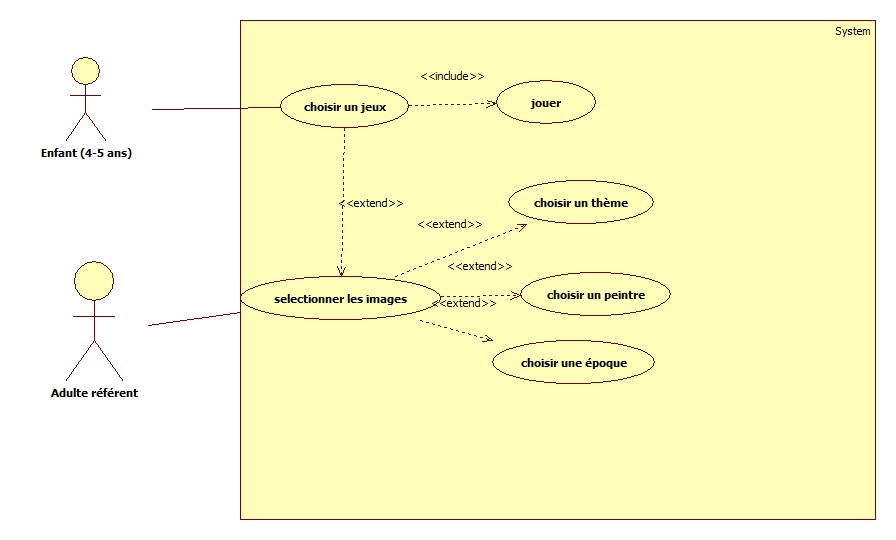
\includegraphics[width=350px]{uml.jpg}
\end{figure}
\subsection{Acteurs}
Enfants et adultes référents
\chapter{Questions à poser au client}
\begin{itemize}
\item C'est qui cet adulte référent?\\
Un adulte référent est un utilisateur (parent ou enseignant) qui permet de créer différentes sessions. Une session est un ensemble d'image préalablement choisis à partir de différents filtre.
\item Faut-il un administrateur?\\
L'administrateur permet de gérer les adultes référents.
\item Niveau des enfants 4, 5 ans?\\
Les enfants ne savent pas lire ni écrire. Il faut donc éviter de leur faire lire des textes ni écrire au clavier.
\item Un référent est il toujours présent lorsque l'enfant joue?\\
Non, l'enfant peut jouer de chez lui mais il sera quand même au moins guidé par ses parents.
\item Référent a un jeux ou plusieurs actifs simultanément?\\
Le référent peut créer plusieurs sessions mais seulement une session peut être activé à la fois (ce qui permet à l'enfant d'arriver directement sur la bonne session sans la sélectionner).
\end{itemize}
\chapter{Idées}
Liste de jeux ;
\begin{itemize}
\item Jeux 94
\item Jeux du pendu
\item Mélange pour facilité (de jeux)
\item Mémo et puzzle
\end{itemize}

\medbreak
Technologies :
\begin{itemize}
\item Utilisation d'un "text to speech" : API Google
\item Utilisation d'un "speech to text" : pas d'API correcte trouvée
\item Base SQL : MySql
\item Utilisation d'un Framework PHP MVC : Laravel
\item Utilisation Framework CSS : Bootstrap
\end{itemize}

\medbreak
Fonctionnement global (prévision) :
\\Page d'accueil : on retrouve les images de profil des référents ayant une session active de jeux.
L'enfant clique sur l'image de son référent et arrive dans le jeux sélectionné par celui-ci.
Le référent peut se connecter afin de créer des sessions de jeux et les activer, les supprimer.\\



\end{document}
